\chapter{Design requirements and approach}\label{cha:solution}

This chapter presents the main goals of the project and the technical specifications. It is also 
intended to give the reader a summary of the proposed functional modules and its structure. 
Any other constraint not mentioned here 
was adjusted or set while being within the design-test loop, as consequence of the prototype nature of the project.
\section{Objectives}
The main goal of this project is to develop a device using open-source tools to read out sensor data from a robot
axis that can be interfaced with an RTE Network. Such that this device can be used afterwards as a test platform 
within an industrial environment to characterize its compatibility with the ongoing IEC/IEEE 60802
TSN Profile for Industrial Automation.

To achieve the main goal the following has to be carried out:
\begin{itemize}
  \item To specify the requirements of the system
  \item Comparison considering the state of the art
  \item To develop the embedded system as a functional EtherCAT Slave Device
  \item To design and manufacture a PCB prototype
  \item To test and report the overall system functionality
\end{itemize}

\section{Technical specifications}

In the table \ref{tbl:tech_specs} the requirements for this project and their state after the implementation can be observed.
This comparison helps as a good summary of the overall achievements that are further detailed in the next chapters.

  \begin{tuhhtable}
    \footnotesize\centering
    \begin{tabular}[hbp]{L{.22\textwidth}L{.22\textwidth}L{.22\textwidth}L{.22\textwidth}}
        \THc{1}{c}{Feature} & \THc{1}{c}{Requirement} & \THc{1}{c}{Implementation} & \THc{1}{c}{Remark} \\
      \abovebodyrule
      \TRh{1}{l}{Upper layer interface}  & Ethernet/EtherCAT compatibility.\newline Non-safety relevant.\newline Services and synchronization: - 
                                        & EtherCAT slave.\newline Services: Mailboxing and CoE\newline Synchronization: Free Run and SM  
                                        & \tblYes\newline FoE and SD synchronization possible in the medium term.\\\TRc
      \TRhc{1}{l}{Display/signaling}    & LED stripes with serial interface:\newline WS2812 \newline 2 Ch  
                                        & 2-4 Ch modifiable in SW\newline Animation capable 
                                        & \tblYes\newline Chs can increase up to number of DMA-Timers (8)   \\
      \TRh{1}{l}{Temperature}           & Data interface for 1-Wire bus     
                                        & 1-Wire Master\newline 15 sensor in bus & \tblYes\newline 6 Sensors simultaneously tested \\\TRc
      \TRhc{1}{l}{PCB}                  & PCB Prototype\newline Layout and size: -   
                                        & Attachable PCB for LAN9252-EVB-SPI.\newline Size: \SI{55 x 38}{\milli\metre} & \tblYes\newline Second layout with both chips included possible in the short term. \\
      \TRh{1}{l}{Safety}                & \tblNA     
                                        & Non Safety-Critical for this prototype & \tblNo\newline FSoE could be researched in the long term.\\\TRc
      \TRhc{1}{l}{Extra interface}      & SPI or I2C interface for current/IMU/black channel   
                                        & Extra SPI considered in PCB and SW\newline JTAG/SWD compatible interface & \tblYes\newline Currently working \\
      \TRh{1}{l}{Speed/position}        & Possible interface of BISS-C type
                                        & Not required for this prototype & \tblNo \\\TRc
      \TRhc{1}{l}{Refresh data cycle}   & -   
                                        & No hard RT deadlines.\newline Deterministic refresh cycle of $\sim$\SI{10}{\milli\second} by RTOS.\newline Timeout faults handling. & \tblGood\newline Timing through RTOS  \\
      \TRh{1}{l}{Data structure}        & -     
                                        & Functional and parametrization data structure as Object Dictionary.\newline Standard ESI file. & \tblYes\newline Currently working\\\TRc
      \TRhc{1}{l}{FW programming}       & -   
                                        & CMSIS - FreeRTOS for thread, event and time management. & \tblGood\newline Currently working \\
      \belowbodyrule
    \end{tabular}
    \caption{Technical specifications;}
    \label{tbl:tech_specs}
  \end{tuhhtable}

Regarding the functional safety features of the device, it is important to mention that, even though this device is considered as non Safety-Critical within
this prototyping stage, the means to create a framework that could be extended to address further reliable development are taken into account, namely
by considering fault tolerance within the software. More comments about this will be done in the results section. 

\section{Solution proposal}
In Fig.~\ref{fig:sysStruct} the proposed layered structure of the functional blocks can be seen, this will help the reader
localize how is the level of interaction of each of the parts that are described along the document. For instance, the project itself 
focuses mainly on the non-dashed blocks; nonetheless, they still need to be configured or adapted according to ACB features. The layered
representation shows three general concepts, namely physical or hardware, middleware and application software. Even though, the blocks
help the reader differentiate between functionalities, most of them are interacting between each other, mostly the Devices' State Machines (DSM).

\begin{figure}[ht]
  \centering
  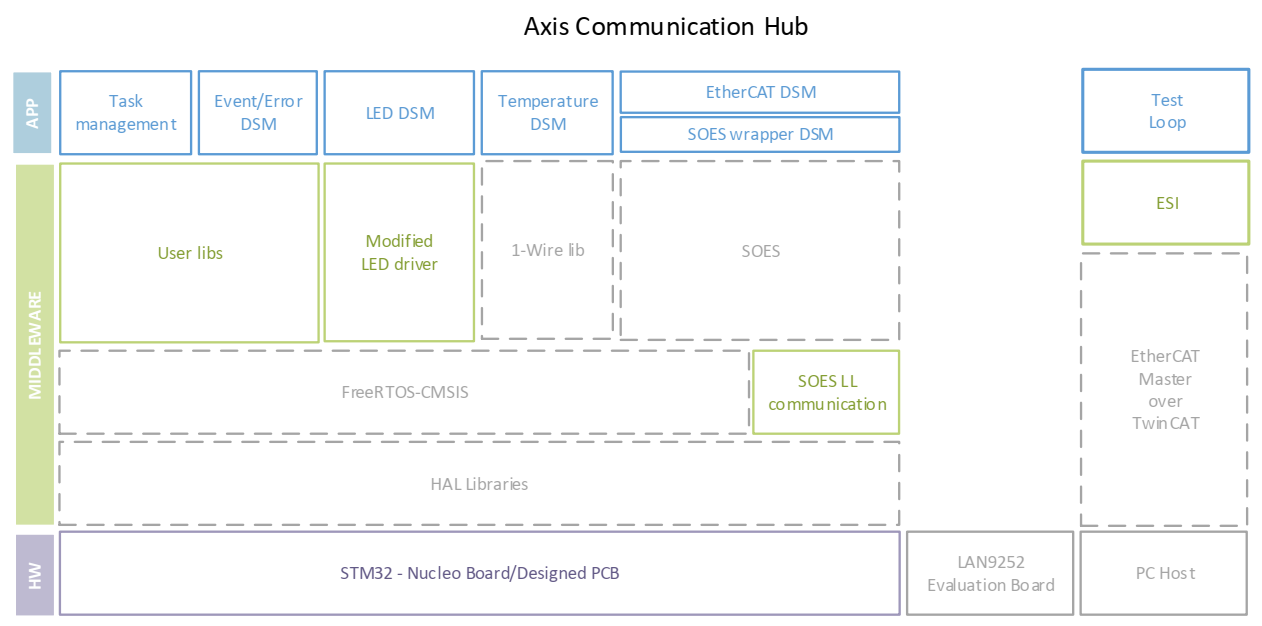
\includegraphics[width=\textwidth]{imgs/prop-system_struct_v2.png}
  \caption{Layered structure of the proposed functional blocks.}
  \label{fig:sysStruct}
\end{figure}

\section{Hardware selection}

In this part it is presented the base hardware that was available to develop the prototype. The microcontroller (MCU) was chosen
due to its active community, resources and current on-develop projects. Other MCUs were though considered, since the overall characteristics
were somewhat similar and generic---regarding peripherals like serial interfaces or Direct Memory Access (DMA) and processing power and memory, for instance.
Therefore, MCUs from Infineon and 
Texas Instruments were good possible candidates---see technical information in ~\cite{infineon_esc},~\cite{infineon_dramfine} and ~\cite{texasi_esc}, respectively; 
however, the basic familiarity with the STM32CubeIDE and the related ST technology 
was a crucial factor. In addition, and concerning the chosen MCU as well, the learning curve is not negligible when it comes to develop any 
firmware at a fair level, even more when it deals with other to-learn
tasks, for instance, development with RTOS, modification of open libraries, EtherCAT protocol itself and the Network Controller chip.

Regarding the Network Controller, the LAN9252 belongs to a set of ASICs that are verified and certified by Beckhoff Automation GmbH. For a further
reference for other alternatives visit ~\cite{beckhoff_esccomparison}. The LAN9252 integrates a so-called EtherCAT Slave Controller (ESC) and it represents a good 
alternative to the Beckhoff's original ASIC ET1100. This way, the basic hardware is there to fulfill Han's Robot Germany's
proposal for developing industrial compatible devices that could enhance the prototyping process within the electronics department. 
Moreover, the mentioned ASIC has a wide compatible control interface that make it be suitable to any microcontroller with which 
the developer has experience. The Table~\ref{tbl:hardware_characteristics} lists the main characteristics of the above mentioned hardware.

\begin{tuhhtable}
    \footnotesize\centering
    \begin{tabular}[tp]{L{.44\textwidth}L{.44\textwidth}}
        \THc{1}{c}{STM32F446ZE} & \THc{1}{c}{LAN9252} \\
      \abovebodyrule
        ARM®32-bit Cortex®-M4 + FPU + Chrom-ART™ Accelerator
        Up to 180MHz CPU\newline
        512 kB of Flash\newline
        128 KB of SRAM
                                        & EtherCAT slave controller with
                                        3 FMMUs and 4 SyncManagers\newline
                                        Distributed clock support\newline
                                        4KB of DPRAM\\\TRc
        General-purpose DMA\newline
        Up to 17 timers\newline
        Up to 4 × I2 C interfaces\newline
        Up to 4 USARTs/2 UARTs\newline
        Up to 4 SPIs\newline
        2 × CAN (2.0B Active)\newline
        USB 2.0 full-speed device/host/OTG 
                                        &100Mbps Ethernet transceivers compliant with IEEE 802.3/802.3u (Fast Ethernet)\newline
                                        8/16-Bit Host Bus Interface, indexed register or multiplexed bus\newline
                                        SPI/Quad SPI\newline
                                        Digital I/O Mode\newline
                                        Multifunction GPIOs
                                        \\
        LQFP64, LQFP100 and LQFP144 packaging     
                                        & Pb-free RoHS compliant 64-pin QFN or 64-pin TQFPEP packaging 
                                        \\\TRc
      \belowbodyrule
    \end{tabular}
    \caption{Summary of the characteristics of both STM32F446ZE and LAN9252 used in the prototype.}
    \label{tbl:hardware_characteristics}
  \end{tuhhtable}

%\subfigbox{
%    \subfigure[NUCLEO-STM32F446ZE]{\label{subfig:stmboard}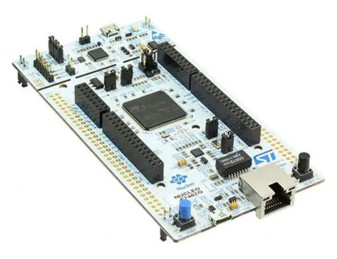
\includegraphics{imgs/sol-stmboard.jpg}}
%    \subfigure[LAN9252-EVB-SPI]{\label{subfig:lanboard}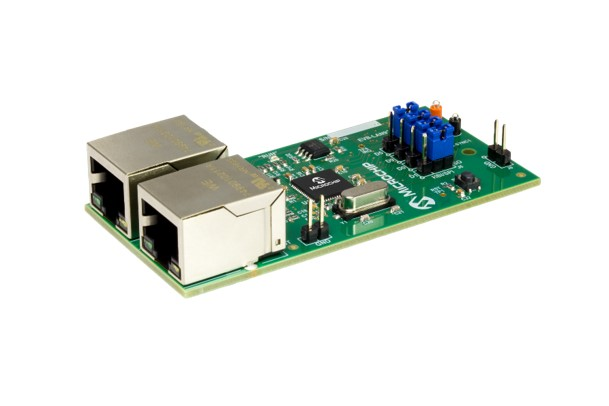
\includegraphics{imgs/sol-lanboard.jpg}}
%}{Evaluation boards for prototyping.}{fig:evalboards}

\begin{figure}[ht]
    \centering
    \subfigure[NUCLEO-STM32F446ZE]{\label{subfig:stmboard}{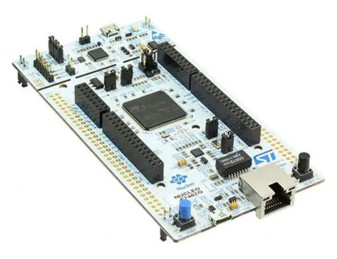
\includegraphics[width=0.4\textwidth]{imgs/sol-stmboard.jpg}}}\hfill
    \subfigure[LAN9252-EVB-SPI]{\label{subfig:lanboard}{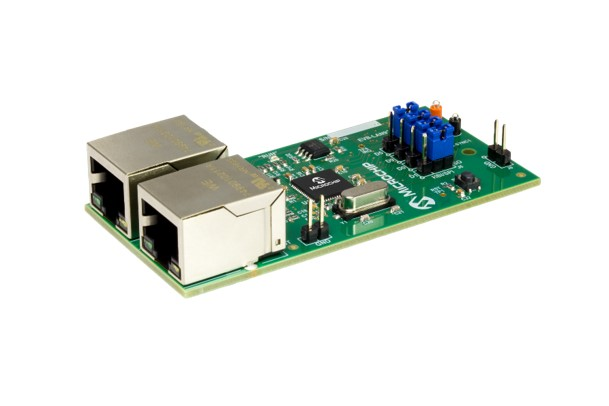
\includegraphics[width=0.4\textwidth]{imgs/sol-lanboard.jpg}}}
    \caption{Evaluation boards for prototyping.}
    \label{fig:evalboards}
\end{figure}

\section{PCB design}\label{sec:pcb_proposal}
As it can be seen in the figure \ref{subfig:lanboard}, the evaluation board includes on-board male pins, this was taken as an advantage and the PCB to be designed
consisted on a pluggable PCB that would be mounted on top of it, increasing minimally the volume already occupied by the evaluation board. This idea needed to be 
designed taking into account the minimum of components based on the Nucleo-STM32F446ZE original design and the requirements of the LAN9252. This means that 
it had to provide, both 5V and 3.3 V power supply, physical ports for the prioritized communication capabilities, minimally SPI, One-Wire JTAG and the LED ports 
according to the technical specifications \ref{tbl:tech_specs}.

\section{Firmware structure}

Since the compatibility with the EtherCAT protocol is the highest priority, all the tasks related to the adjustment of existing libraries and 
the synchronization between them are also prioritized, such that the main functionality can operate. Taking this into consideration and 
recalling the final proposal for the structure of the embedded system, Fig.~\ref{fig:sysStruct}, the functional blocks are represented differently. 
The ones in gray or dashed lines are mainly components that are planned not to be modified
at all or not in deep, because of either its complexity or its given reliability. This means, its functionality is almost granted. 
Nevertheless, the progress relies on documentation that can be either good or poor, for instance, TwinCAT has good resources, 
whereas SOES does not. Regarding the latter, the block refers to the main library to be integrated, that enables the EtherCAT features; 
although, 
it is represented with dashed-lines, it was changed but not restructured.
However, detailed information about these concerns are presented along the implementation and result chapters.

The word firmware rather generalizes the set of written/modified code that needs to be carried out through the implementation, for instance, the
top layer in blue corresponds to the application-related source files written in C, while the Test loop executes over TwinCAT3 and is written
in SText, which needs mandatory an EtherCAT Slave Information (ESI) file written in XML. The name middleware, in this case, represents not 
only the Hardware Abstraction Layer (HAL) libraries provided by STM, nor the CMSIS-RTOS's, but also represents the user-define libraries for each
DSM and the modified libraries, namely those for the LED and One-Wire---as well as the already mentioned case of SOES. This structure is important to have
in mind, mainly while going through the implementation chapter.

Additionally, another thing to consider within this document is the abbreviation \emph{DSM} (Device's State Machine) which is used as substitute for State Machine,
such that it is not confused with Synchronization Manager, defined as well by Beckhoff Automation as SM.



%TODO this figure needs to be updated changing the Error handler to Event handler, configuration/management to auxiliar functions --monitor for debugging
%adding as well the ESI file as a functional block running on top of the LAN9252 Evaluation board
%Where could I mention about the wrappers used to integrate the functions contained within the 3rd party libraries and my SMS?